\subsubsubsection{curve-scalar}

\begin{enumerate}
    \item \verb|Target|: Implement the multiplication between scalar and point.
    \item \verb|Constraints logic|: See \figref{fig:curve-scalar}.
    \item \verb|Constraints info and costs|:
    \begin{itemize}
        \item gate type num: 13 
        \item gate instance num: 180364          
    \end{itemize}
\end{enumerate}

\begin{figure}[!ht]
    \centering
    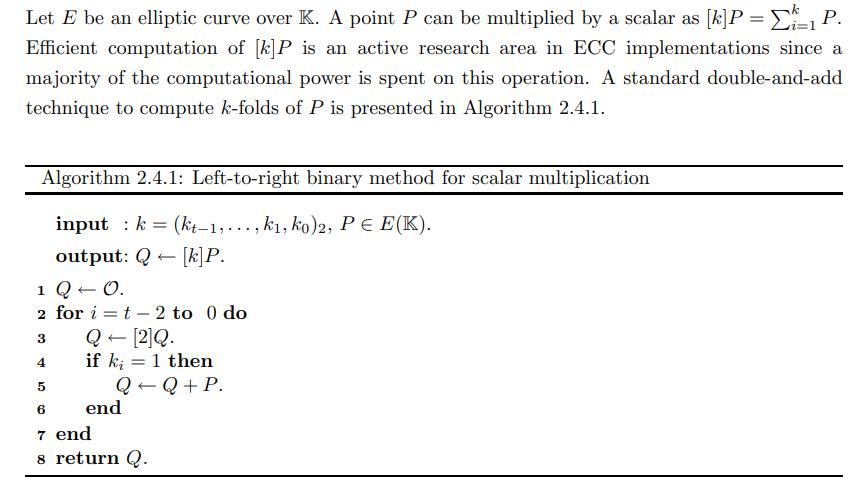
\includegraphics[width=0.6\textwidth]{curve-scalar.jpg}
    \caption{curve-scalar}
    \label{fig:curve-scalar}
\end{figure}
